\documentclass[conference]{IEEEtran}
\IEEEoverridecommandlockouts
% The preceding line is only needed to identify funding in the first footnote. If that is unneeded, please comment it out.
\usepackage{cite}
\usepackage{amsmath,amssymb,amsfonts}
\usepackage{algorithmic}
\usepackage{graphicx}
\usepackage{textcomp}
\usepackage{xcolor}
\usepackage{float}
\def\BibTeX{{\rm B\kern-.05em{\sc i\kern-.025em b}\kern-.08em
    T\kern-.1667em\lower.7ex\hbox{E}\kern-.125emX}}
\begin{document}

\title{Longitudinal Feature Extraction in International Logistics Performance Index
}

\author{\IEEEauthorblockN{Aldina Correia}
\IEEEauthorblockA{\textit{CIICESI, ESTG, Instituto Politécnico do Porto} \\
Felgueiras, Portugal \\
aic@estg.ipp.pt, 0000-0002-4693-4867}
\and
\IEEEauthorblockN{Diogo Ribeiro}
\IEEEauthorblockA{\textit{Data Science and Research} \\
\textit{MySense}\\
London, United Kigdom \\
diogo.ribeiro@mysense.ai, 0009-0001-2022-7072}
}

\maketitle

\begin{abstract}
 The importance of the logistics performance of companies, regions and countries to support decision-making is universally recognised, covering the rationalisation of supply chains, the optimisation of inventory management and promoting global collaboration. 
      
  Efficient logistics integration with innovative technologies is crucial for the prompt delivery of materials and components, increasing the speed and effectiveness of innovation processes and, consequently, the performance of organisations. This study examines the robust correlation structure between Logistics Performance Index (LPI) indicators over several years. 
  %
  The LPI assesses global logistical performance by measuring factors such as the quality of commercial and transport infrastructure, the ease of customs procedures and the efficiency of customs clearance, among other aspects that influence the transnational flow of goods.

Our results confirm the LPI as a longitudinal latent variable, characterised by its indicators, which demonstrate remarkable internal consistency. This consistency underpins the reliability of the LPI for assessing global logistics performance.
%
Recognised as a valuable measure of logistics efficiency, LPI serves as a practical tool in business and politics, guiding strategic decision-making and improving the operational cost-benefit ratio and competitiveness of organisations.
\end{abstract}

\begin{IEEEkeywords}
component, formatting, style, styling, insert
\end{IEEEkeywords}

\section{Introduction}
The speed and efficiency with which companies transport goods across international borders, thanks to globalisation, have become fundamental characteristics of their global competitiveness. This encourages the continued development of performance measures such as the
 World Bank’s Logistics Performance Index (LPI) \cite{beysenbaev2020}, Global Competitiveness Index (GCI) \cite{wef2020}, Global Enabling Trade Index (GETI) \cite{wef2018} and UNCTAD Liner Shipping Connectivity Index \cite{unctad2020}. Access to these measures quickly, automatically and efficiently is crucial \cite{babayigit2023, shepherd2023}. 


%\textcolor{red}{Frases completas de 1 fonte?}
LPI, measures the performance of countries logistics system and provides a guide for businesses and policymakers interested in global trade and international investments \cite{arvis2016,arvis2018,arvis2023,civelek2015}. The LPI allows countries to assess their current logistics-related strengths and weaknesses, identifying the areas in which they need to improve, and benchmark their performance against global standards, to enhance their international trade capabilities \cite{beysenbaev2020,polat2023}.

Improving the LPI requires a broad and coordinated approach that addresses various factors impacting a logistics system, simplifying and standardising in customs procedures and regulations can significantly reduce the time and cost associated with clearing goods at the border \cite{babayigit2023,beysenbaev2020}. Investment in transport infrastructure, the diversification of international transport options, and the optimisation of transportation methods improve the connectivity, reliability, flexibility, and accessibility of logistics networks \cite{marti2014}. Further investment in human resources, new technologies and innovation is crucial to increase the quality and competence of logistics services. The adoption of digital platforms and tools for better tracking and tracing improves the visibility and security of cargo movements, moreover, reducing variability and uncertainty in logistics operations decreases the probability of failures in delivery \cite{WBreport2018}.

%\textcolor{red}{FONTE???}
The relevance of the LPI fundamentally derives from its ability to reflect the nuances of a nation's logistics system — a crucial element for trade effectiveness, economic dynamism and comprehensive social progress \cite{rezaei2018, sharif2024}. Nations with high LPI scores often demonstrate more efficient logistics, which not only speeds up the transportation of goods but also strengthens competitiveness and access to markets \cite{worldbank4}. Conversely, low LPI scores can indicate underlying problems, such as high costs, operational delays and significant risks, that can diminish a country's attractiveness in the global trade landscape \cite{arvis2016,arvis2018,arvis2023}. The LPI transcends its function as a simple metric, being crucial for monitoring the effectiveness of logistics reforms and investments, providing policymakers with a tool to assess the impact of strategic changes on national performance \cite{worldbank5}. 

This paper aims to validate the LPI as a reliable measure of logistical performance by analysing key characteristics and relationships among its indicators. Recognising the LPI as a robust metric allows it to inform strategic decision-making in engineering and other sectors, improving operational cost-effectiveness and competitiveness. Additionally, the paper tracks Portugal’s LPI performance from 2007 to 2023, focusing on its changes and implications for logistics strategy.

This paper seeks to validate the LPI as a measure of logistical performance by analysing key characteristics and relationships among its indicators. By recognising the LPI as a feasible and robust metric, it can be employed to inform strategic decision-making across business, logistics, and policy sectors, thereby enhancing operational efficiency and competitiveness on a global scale.
For that Principal Component Analysis (PCA) is considered for extracting the essential feature in the data.

The structure considered is divided into four sections. In the first the theme and importance of the LPI index are presented, in the second the main concepts of PCA are highlighted, the third encompasses the data analysis and presents the results obtained, and the fourth consists of the conclusion and future work of the study.


\section{Principal Component Analysis}

Principal Component Analysis (PCA) is a robust statistical tool utilised extensively in data analysis and machine learning to identify patterns in data and express the data in such a way as to highlight their similarities and differences. Since its establishment, PCA has been widely applied to reduce the dimensionality of large data sets, enhancing interpretability while minimising loss of important information \cite{jolliffe2016principal, monahan2000nonlinear, takane2001constrained, maroco2018, watkins2018}.

PCA provides a comprehensive explanation of the global dataset, retaining the maximum variability in the data and minimising the number of features extracted, which is advantageous for effective analysis.

There are several compelling reasons to consider transforming a dataset into a lower-dimensional space, such as simplifying data manipulation and reducing computational demands \cite{wang2003feature, wu2007feature, correiaICIE}. However, it is critical to do this transformation systematically, as reducing dimensions can result in a loss of information. It is essential that the chosen algorithm retains the valuable PCA could be introduced from different viewpoints, elucidating why it is advantageous to preserve maximal variability in the data \cite{hasan2021review, ivosev2008dimensionality, bro2014principal}.

The mathematical foundation of PCA is based on the linear algebra concepts of eigenvalues and eigenvectors \cite{wold1987principal}. PCA transforms the original variables into a new set of variables, which are linear combinations of the original variables. These new variables, or principal components, are obtained by orthogonal transformation directed along the axes of maximum variance.

The covariance matrix of the initial data is defined as:
\[
\Sigma = \frac{1}{n-1} \sum_{i=1}^{n} (x_i - \mu)(x_i - \mu)^T
\]


The principal components are derived from the eigenvectors of the covariance matrix of the data, scaled by their respective eigenvalues. The first principal component is the direction along which the variance of the data is maximised.

The eigenvalue equation is given by:
\[
\Sigma v = \lambda v,
\]
where $\Sigma$ represents the covariance matrix, $v$ denotes an eigenvector matrix, and $\lambda$ is the corresponding eigenvalue vector.

%\textcolor{red}{Só há 1 $V$?}

Dimensionality reduction is achieved by selecting the top $k$ principal components, corresponding to the largest eigenvalues (usually greater than 1), which capture the most significant variance within the dataset. This truncation allows for a lower-dimensional representation of the data, which retains the core characteristics of the original dataset \cite{shlens2014tutorial}.

The data projection can be expressed as:
\[
Y = X \cdot V_k,
\]
wWhere $X$ is the original data matrix, $V_k$ is the matrix containing the top $k$ eigenvectors, and $Y$ represents the transformed data with reduced dimensions.

The application of PCA is not limited to dimensionality reduction. It also is as a powerful tool for noise reduction, feature extraction, and data visualisation. By simplifying complexity in high-dimensional data, PCA facilitates a clearer understanding of the data's underlying structure \cite{ivosev2008dimensionality}.

\subsection{Applications of PCA}

PCA is extensively utilised in various analytical scenarios requiring the reduction of data dimensionality and the extraction of significant patterns from the data \cite{wang2003feature}. The utility of PCA extends across several key domains:
\begin{itemize}
    \item PCA is particularly valuable in scenarios involving datasets with numerous variables. By identifying and eliminating redundant or less important variables, PCA simplifies the dataset while preserving the most crucial information, thus facilitating more efficient further analyses \cite{wu2007feature}.
    \item For high-dimensional data, PCA provides a mechanism to reduce dimensions to two or three principal components. This reduction allows for the visual representation of complex structures, making the data more comprehensible and easier to interpret \cite{hasan2021review}.
    \item In datasets characterised by high levels of noise, PCA enhances data quality by focusing on principal components that capture the core variance of the data, which are less influenced by noise \cite{ivosev2008dimensionality}.
    \item In predictive modelling tasks, PCA is employed to derive new features that potentially offer greater insight and less redundancy than the original set of features\cite{wang2003feature}.
    \item PCA serves as a powerful exploratory tool, helping to uncover hidden variables and detect unusual patterns within the data, which might not be apparent through traditional analysis methods \cite{wu2007feature}.

\end{itemize}







\subsection{Key Assumptions of PCA}
PCA serves as an influential statistical method extensively employed to reduce dimensionality in data analysis. Nonetheless, the success of PCA depends on certain assumptions regarding the data it handles. Understanding these assumptions is essential to guarantee that PCA's application yields significant and dependable outcomes \cite{bro2014principal, shlens2014tutorial, wold1987principal, candes2011robust, mckeown1998independent}.

Key Assumptions of PCA are:

\begin{itemize}
    \item \textbf{Linearity:} PCA assumes that the data components have linear relationships among them. This assumption is fundamental because PCA aims to capture the variance through linear combinations of the original features. It implies that the principal components derived from PCA are linear transformations of the original variables. This assumption also means that PCA may not effectively capture complex nonlinear relationships without transformations or adaptations.
    
    \item \textbf{Scale Sensitivity:} The scale of the data matters in PCA because it directly influences the resulting principal components. Variables with larger variances can dominate the outcome, overshadowing the contributions of other variables. Therefore, it is often necessary to standardise or normalise (or re-scaling) data before applying PCA, so each variable contributes equally to the analysis.
    
    \item \textbf{Large Variance Implies Importance:} PCA operates under the assumption that directions in which the variance of the data is maximised are the most important. The technique prioritises these directions to identify the principal components. This assumption may not always hold true, especially in cases where high variance is due to outliers or noise in the data.
    
    \item \textbf{Orthogonality of Components:} PCA assumes that the principal components are orthogonal, meaning each component is uncorrelated with the others. This orthogonality ensures that the principal components represent independent dimensions of variance, simplifying the interpretation of the data by removing redundant information.
    
    \item \textbf{Normality:} While not strictly required, PCA ideally assumes that the data follows a multivariate normal distribution. This assumption helps in maximising the efficiency and interpretability of PCA, particularly when using PCA results for further statistical inference. The normality assumption is imperative for the application of various statistical tests that may be needed to evaluate the results of PCA.
    
    \item \textbf{Sample Size:} PCA assumes that there is an adequate sample size to reliably estimate the covariance matrix. A small sample size may lead to over-fitting, where the PCA model captures noise instead of the underlying data structure. Generally, a larger sample size provides a more stable and accurate estimation of covariance, leading to more reliable PCA results.
\end{itemize}

When applying PCA, it's crucial to assess whether these assumptions hold for the given dataset. Violations of these assumptions can lead to misinterpretations and misleading conclusions. For instance, if the data is not linear, using kernel PCA or another nonlinear method might be more appropriate. If components are not orthogonal due to the presence of multicollinearity, PCA might still reduce dimensionality, but the interpretation of components becomes more complex.

While PCA is a robust and versatile tool in data analysis, careful consideration of its underlying assumptions is essential to utilise its full potential effectively. Ensuring that these assumptions are met or appropriately addressed through pre-processing steps can greatly enhance the insights gained from PCA.


\subsection{Validating PCA}

To ensure the effectiveness of PCA in specific contexts, several validation steps are recommended, \cite{bro2014principal, shlens2014tutorial, wold1987principal, candes2011robust, mckeown1998independent}:

\begin{itemize}
 \item \textbf{Optimal number of principal components to retain:}
\begin{itemize}  \item \textbf{Scree Plot Analy} -- Initiate the validation by examining, for example, the eigenvalues of the covariance matrix through a scree plot. This plot is crucial for suggest the optimal number of principal components to retain, typically identified by the point where the explained variance ceases to decrease significantly.
  \item \textbf{Variance Explained:} Quantify the amount of variance each principal component accounts for. The objective is to retain a minimal number of components while capturing a substantial proportion of the data's total variance, with common thresholds ranging from 70\% to 90\%.
  \item \textbf{Data investigation area} -- Theoretical investigation in the theme of the data, can suggest the more adequate theoretical number of factors.
\end{itemize}
  \item \textbf{Loadings Examination:} Analyze the loadings of each principal component to understand the relationships and contributions of the original variables to the components. This analysis can highlight the most significant variables within the dataset.
  \item \textbf{Cross-Validation:} If PCA is applied within predictive modeling, cross-validation should be performed to compare the efficacy of models using both the original and reduced datasets. This step ensures that the reduction process does not omit critical information.
  \item \textbf{Reconstruction Error:} Calculate the reconstruction error, which is the discrepancy between the original dataset and its reconstruction from the selected principal components. A minimal reconstruction error indicates effective information retention by the principal components.
  \item \textbf{Qualitative Evaluation:} Assess the practicality of the PCA-reduced dataset for the intended application. Considerations should include the balance of variable importance, as over-simplification could result in the loss of essential information.
\end{itemize}

\subsection{Statistical Tests for PCA Suitability}

Prior to executing PCA, it's important to perform statistical tests to determine if the data is appropriate for such analysis:

\begin{itemize}
    \item \textbf{Bartlett’s Test of Sphericity:} This test checks if the correlation matrix significantly deviates from an identity matrix. A significant result implies that the conditions are favorable for PCA.
    \item \textbf{Kaiser-Meyer-Olkin (KMO) Test:} This test measures the suitability of data for factor analysis, which also reflects on its appropriateness for PCA. A KMO value above 0.6 is considered adequate, with values approaching 1.0 being optimal.
    \item \textbf{Measure of Sampling Adequacy (MSA):} Within the KMO test, the MSA score is calculated for each variable to assess individual suitability. Values below 0.5 generally suggest that the variable is not suitable for PCA.
\end{itemize}

\section{Data and Results}
The LPI \cite{worldbank2024} is an aggregate index for a welfare evaluation of countries’ logistics performance worldwide based on multiple variables. The LPI is derived from a survey of international freight forwarders and express carriers around the world and is an overall impression of countries’ performance in six key dimensions \cite{WBreport2016,WBreport2018}:
\begin{enumerate}
    \item \textbf{Customs} Clearance Process: The efficiency of customs and border clearance processes.
    \item \textbf{Infrastructure} Quality: The quality of trade and transport-related infrastructure, including ports, railroads, and roads.
    \item Ease of Arranging \textbf{(International) Shipments}: The ease of arranging competitively priced shipments.
    \item \textbf{Logistics Competence and Quality } of Services: The competence and quality of logistics services, such as transport operators and customs brokers.
    \item \textbf{Timeliness} of Shipments: The frequency with which shipments reach the consignee within the scheduled or expected delivery time.
    \item \textbf{Tracking and Tracing}: The ability to track and trace consignments.
\end{enumerate}
 The scores for each of these aspects of logistics performance are weighted averages of country scores and hard data that capture logistic efficiency by quantifying the ease with which goods cross borders and circulate in the country, that is, to allow goods to flow into, and to transit within, the country in a speedy and cost-efficient manner.

To identify the variables that most contribute  to the countries' logistical performance, techniques for selecting or extracting key indicators can be used. In both cases, the aim is to retain the indicators that maximise the variance extracted from the original data.

In \cite{correiaICIE}, to ensure that the extracted characteristics were relevant and informative in relation to the 2023 Logistics Performance Index indicators, extraction techniques were used, in particular Exploratory Factor Analysis (EFA), using PCA in the JASP \cite{JASP} software.

The present study considers LPI indicators over several years, being therefore a longitudinal approach, using the software R \cite{R}.

This analysis is based on the values of the LPI \cite{lpi_worldbank_2023} indicators in the years 2007, 2010, 2012, 2014, 2016, 2018 and 2023.

As the EFA carried out in \cite{correiaICIE} allowed the identification of a single factor, in this work a Principal Component Analysis (PCA) was carried out over the available years, considering one component.

Assumptions for this techniques (EFA and PCA)  are: (i) sample dimension -- 5 to 10 observations by variable; (ii) normality of the variables; (iii) linearity of the variables; (iv) homocedasticity.

(i) Sample dimension - The sample comprises between 139 and 160 countries (Table \ref{tab:kmo}), and there is no missing values. Therefore, the sample size is adequate for the analysis of the six indicators.

\begin{table*}[h]
  \caption{Kaiser-Meyer-Olkin and MSA}
  \label{tab:kmo}
  \centering
\begin{tabular}{lccccccc}
\hline
\textbf{Indicator (Score)}	&	\textbf{2007}	&	\textbf{2010}	&	\textbf{2012}	&	\textbf{2014}	&	\textbf{2016}	&	\textbf{2018}	&	\textbf{2023}	\\  
\hline
Customs	&	0.91	&	0.92	&	0.93	&	0.89	&	0.95	&	0.95	&	0.91	\\	
Infrastructure	&	0.90	&	0.88	&	0.94	&	0.91	&	0.93	&	0.92	&	0.90	\\	 
International Shipments	&	0.96	&	0.98	&	0.96	&	0.97	&	0.96	&	0.96	&	0.97	\\	 
Logistics Competence and Quality	&	0.93	&	0.89	&	0.91	&	0.91	&	0.93	&	0.91	&	0.93	\\	 
Timeliness	&	0.97	&	0.98	&	0.96	&	0.94	&	0.94	&	0.96	&	0.94	\\	 
Tracking and Tracing	&	0.93	&	0.94	&	0.94	&	0.93	&	0.94	&	0.95	&	0.92	\\	 
\hline
KMO - Overall MSA	&	0.93	&	0.92	&	0.94	&	0.92	&	0.94	&	0.94	&	0.93	\\	 
\hline
Number of Countries	&	150	&	155	&	155	&	160	&	160	&	160	&	139\\	
\hline
\end{tabular}
\end{table*}

(ii) Normality Assessment - Both the Mardia Test and the Energy Test were used, under the null hypothesis of multivariate normality.
In some year Mardia's Test presented p values greater than 0.05, therefore, a multivariate normal distribution can be considered, but in most years none of the tests allows to confirm this assumption.

(iii) Linearity -- Pearson's Correlations between Indicators are significant at the 5\% significance level, in addition, they are all high, exceeding the value of 0.8, suggesting a strong interdependence between them (multicollinearity).
Consequently, the extraction of factors from these characteristics is justified and imperative, in order to exclude potential redundancies and increase the robustness of the analysis.

(iv) Homoscedasticity -- The standard deviation values of the indicators are close to and below 1, which suggests the existence of homoscedasticity and a relatively consistent distribution of data around the respective means for each indicator, over the years.

Once the necessary conditions have been verified, PCA can be implemented to extract the principal component that maximises the retention of variance of the observed variables.

%----- Requires booktabs package -----%
The Kaiser-Meyer-Olkin (KMO) Measure of Sample Adequacy (MSA) or Overal MSA and the MSA for each variable indicates the suitability of the variable for PCA. 

KMO ranges between 0.92 and 0.94, over the years
and the individual MSA of each variable between 0.88 and 0.98.
This all individual MSAs are greater than the 0.5 threshold, indicating that they are adequate for the analysis. Additionally, the overall MSA or KMO  values suggests excellent suitability for applying PCA \cite{maroco2018analise}. 


%\textcolor{red}{FALTAM OS RESULTADos}
%The chi-square goodness-of-fit test, with null hypothesis that the observed data correlation matrix  is a random sample realisation from population having correlation matrix equal to the one returned by the extracted factors, has the $\chi^2$ presented in Table \ref{tab:loadings}, with $df=9$ and a $p-value <0.001$.

In determining the number of factors to retain by focusing on PCA eigenvalues  exceeding 1 (\cite{carroll1978effect}), a single factor was extracted  over the years. The percentage of variance retained of these indicators over the years is between 87.8 and 94.4 (Table \ref{tab:loadings}). 
This means that all indicators contribute to the same latent variable, indicating a high level of correlation between them.

Within this factor,  \textit{Logistics Competence and Quality} is always the indicator with highest loading. The behaviour of the loading's values across the time can be observed in Table \ref{tab:loadings} and Figure \ref{fig:PCAl} and are between values 0.86 and 0.98.

\begin{figure*}
    \centering
    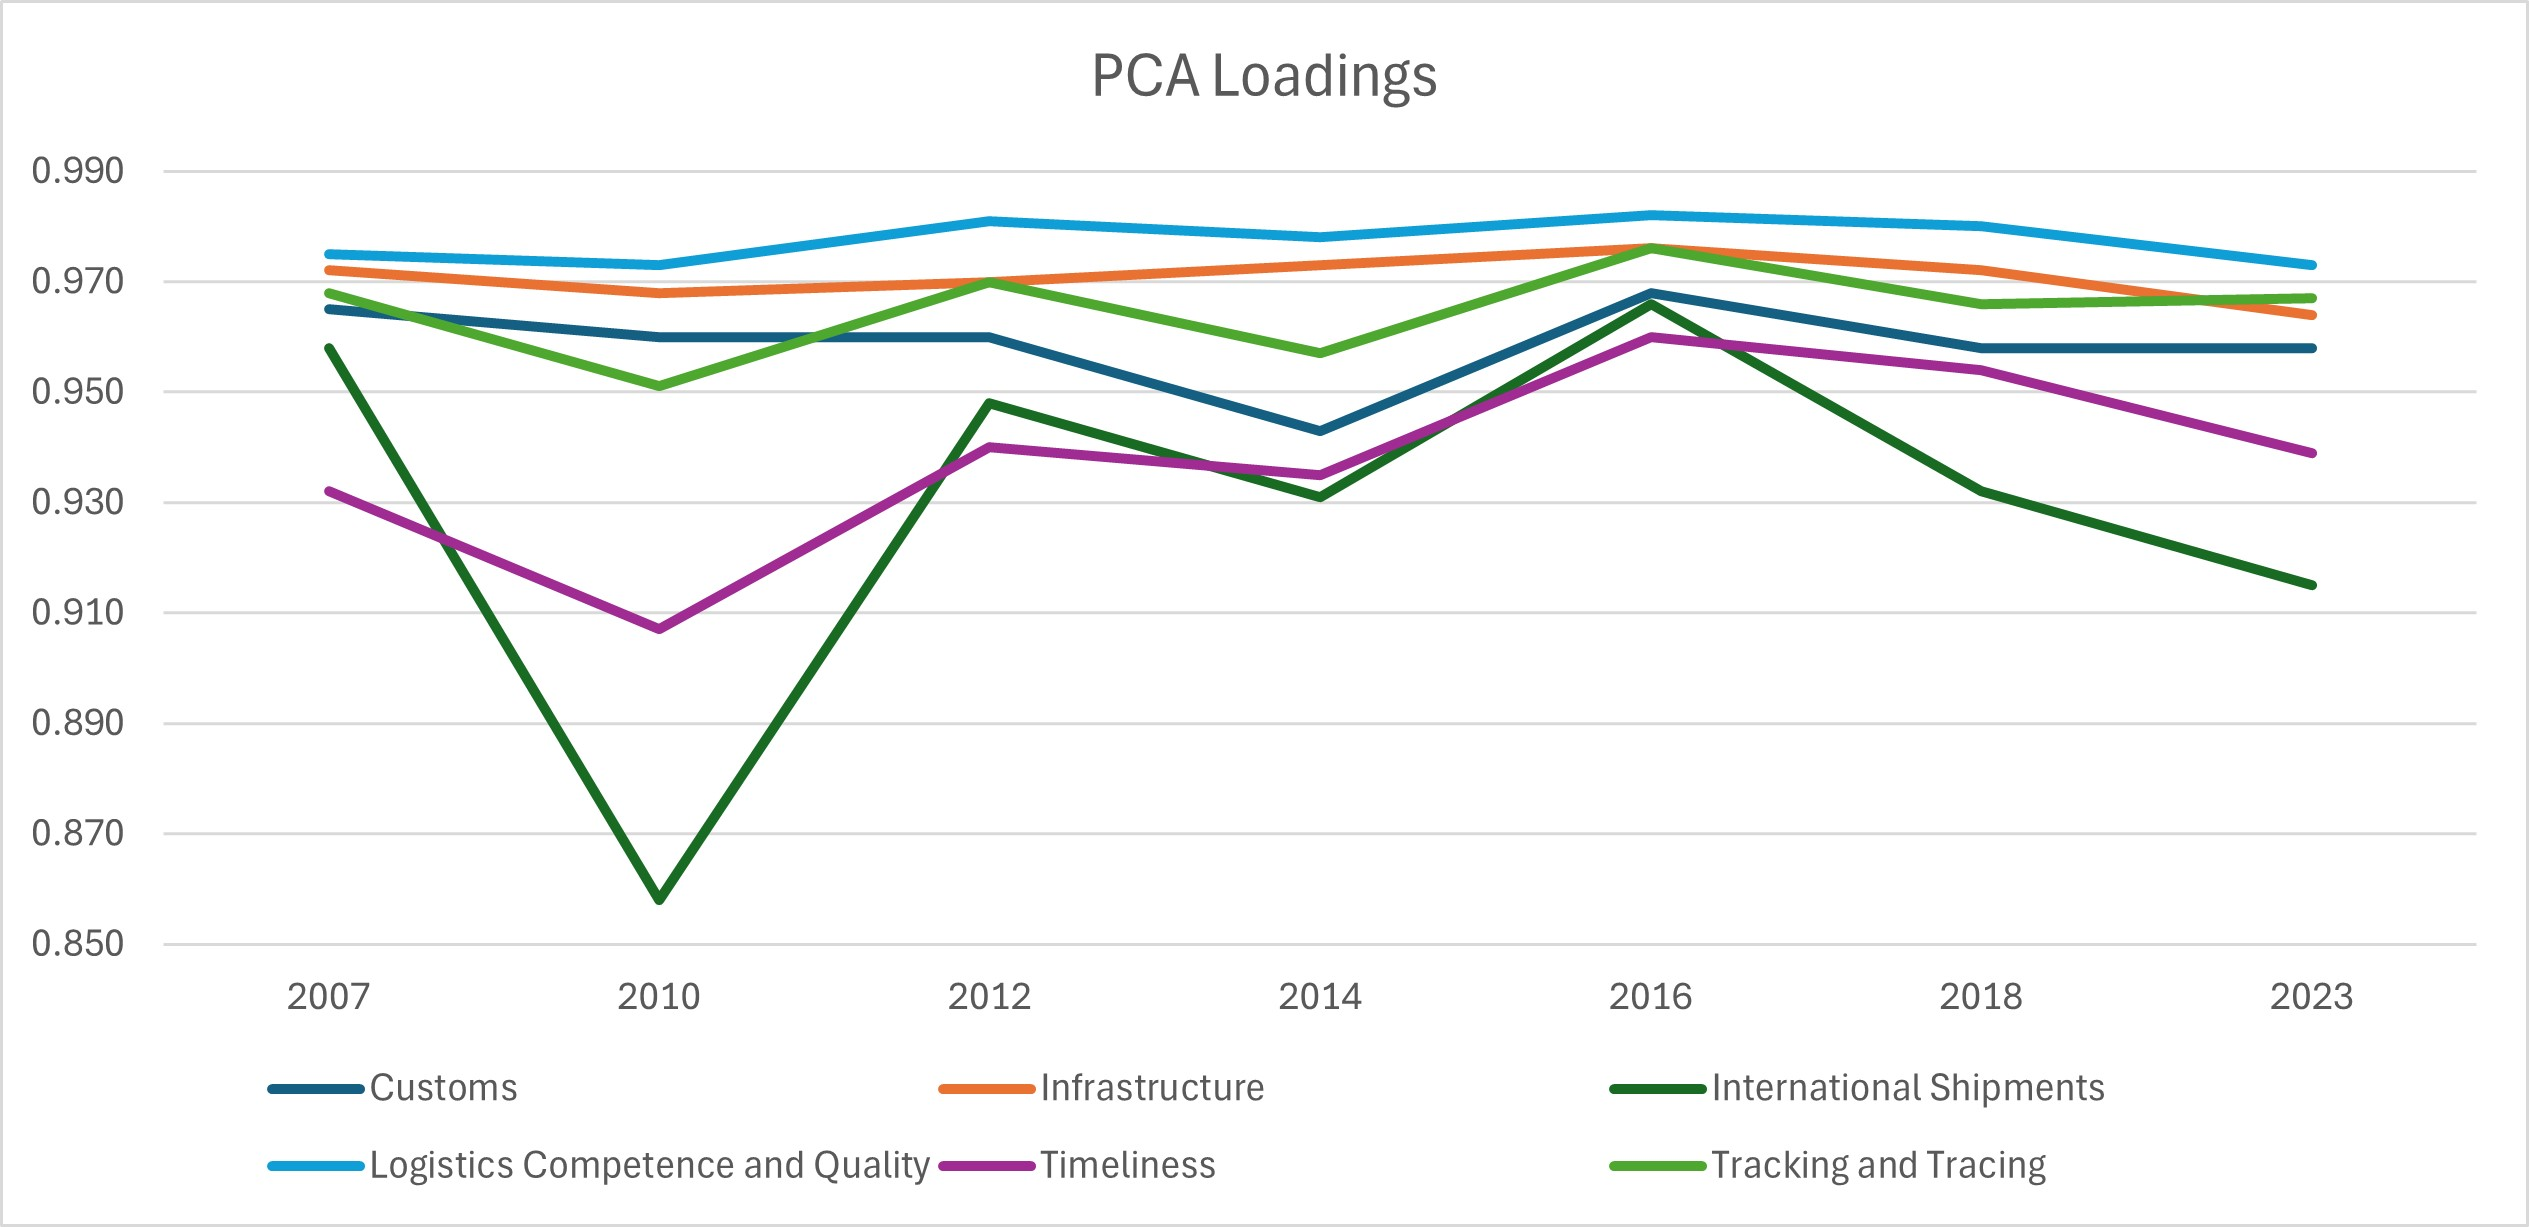
\includegraphics[width=0.7\textwidth]{Loadings.jpg}
    \caption{PCA Loadings across the years}
    \label{fig:PCAl}
\end{figure*}

The \textit{Infrastructure} indicator presented the second highest value since 2007, but was surpassed by \textit{Tracking and Tracing} in 2023.

The \textit{Customs} indicator has shown almost constant behaviour over the years, generally appearing in third or fourth position, in relation to loading values.

The indicators with lower values were \textit{Timeliness} and \textit{International Shipments}, particularly in 2010.

Since 2016, the loading's of all indicators have been decreasing.

%The reliability of factors in the context of factor analysis refers to the consistency or stability of the measurement of underlying constructs represented by those factors. There are several ways to assess the reliability of factors, being the commonly used measure the Cronbach's Alpha, a frequentist scale Reliability Statistics. It assesses how well the items within a factor consistently measure the same underlying construct. A higher Cronbach's alpha value (typically above 0.70) indicates greater reliability.
%


\begin{table*}[h]
  \caption{PCA Loadings, Explaned Variance and Reliability}
  \label{tab:loadings}
  \centering
\begin{tabular}{lccccccc}
\hline
\textbf{Indicator (Score)}	&	\textbf{2007}	&	\textbf{2010}	&	\textbf{2012}	&	\textbf{2014}	&	\textbf{2016}	&	\textbf{2018}	&	\textbf{2023}	\\  
\hline
Customs	&	0.965	&	0.960	&	0.960	&	0.943	&	0.968	&	0.958	&	0.958	\\	
Infrastructure	&	0.972	&	0.968	&	0.970	&	0.973	&	0.976	&	0.972	&	0.964	\\	
International Shipments	&	0.958	&	0.858	&	0.948	&	0.931	&	0.966	&	0.932	&	0.915	\\	
Logistics Competence and Quality	&	0.975	&	0.973	&	0.981	&	0.978	&	0.982	&	0.980	&	0.973	\\	
Timeliness	&	0.932	&	0.907	&	0.940	&	0.935	&	0.960	&	0.954	&	0.939	\\	
Tracking and Tracing	&	0.968	&	0.951	&	0.970	&	0.957	&	0.976	&	0.966	&	0.967	\\	\hline
Explaned Variance (\%) - 1 factor 	&	92.5	&	87.8	&	90.8	&	92.4	&	94.3	&	92.3	&	90.8	\\	\hline
Reliability - Cronbach' $\alpha$	&	0.983	&	0.970	&	0.982	&	0.979	&	0.987	&	0.982	&	0.978	\\	\hline
\end{tabular}
\end{table*}

The estimate Cronbach's $\alpha$ of the factor obtained across the time is between $0.970$ and $0.987$, indicating excellent reliability. This provides evidence of the excellent internal consistency of the latent variable.

Cronbach's $\alpha$ of the extracted component obtained over time under analysis is between $0.970$ and $0.987$, indicating excellent reliability. This provides evidence of the excellent internal consistency of the latent variable over the years.

\section{Conclusion and Future Work}

In this study it is concluded that there is a strong correlation between all LPI indicators over the years, suggesting a good definition of the LPI as latent variable. This correlation structure remains almost unchanged over the time, with the main indicator always being the same over the years. In fact, the positioning of the loadings of all indicators is at values above 0.85, therefore all of them are very close to 1.

The LPI also presents a notable internal consistency over the years, meaning the high level of correlation between these indicators, which  implies a coherent and unified measurement of the latent variable, reinforcing the reliability and coherence of the LPI as a robust tool for evaluating logistics performance.

This vision contributes to an understanding of logistics performance and can be generalized to organizations as a reference measure on a national and global scale, guiding the decision-making and strategic decisions with regard to the logistics performance of organizations, regions and countries.

A good suggestion for future work is to develop a logistics performance index for logistics companies and extending these concepts to the industrial level. This would be very useful for these companies. 

Another suggestion is to consider a Longitudinal approach to PCA, using for example the R package \cite{jarmund2022alasca} and also a model based clustering and dimensionality reduction of mixed data \cite{ranalli2017model} approach.




\section*{Acknowledgment}

This work has been supported by national funds through FCT - Fundação para a Ciência e Tecnologia through project UIDB/04728/2020.

%\section*{References}



\bibliographystyle{ieeetr}
\bibliography{sample-base.bib}

\end{document}
